\begin{pastexam}[label={px:ccu-115-swa-04}]{中正資工所甲組 115 學年度 第 14 題}
（複選；全對才給分）

(10\%) (\qquad) Given a simple graph $G(V,E)$ $with$ $V=\{A,B,C,D,E,F,J,H,I\}$,
\[\begin{aligned}E=\{&(A,B),(A,F),(A,J),(B,C),(B,D),(B,E),\\&(B,J),(C,D),(E,F),(J,I),(J,H),(I,H)\},\end{aligned}\]
What are the biconnected components?\\
(a)~$\{A,B,C,D\}$ \qquad (b)~$\{B,C,D\}$ \qquad (c)~$\{A,B,E,F\}$ \qquad (d)~$\{G,H,I\}$\\
(e)~none of the above
\end{pastexam}

\begin{pastsoln}
答案：(b)。

先說原題的問題：頂點集合裡沒有 G（原本字母順序上 G 的位置寫成了 J），選項 (d) 卻寫
$\{G, H, I\}$。 照字面，圖裡沒有 G，(d) 不是雙連通元件，答案只有 (b)；如果出題者的意思是
$\{J, H, I\}$，那 (d) 也對，答案是 (b)(d)。 下面照字面作答。

\begin{center}
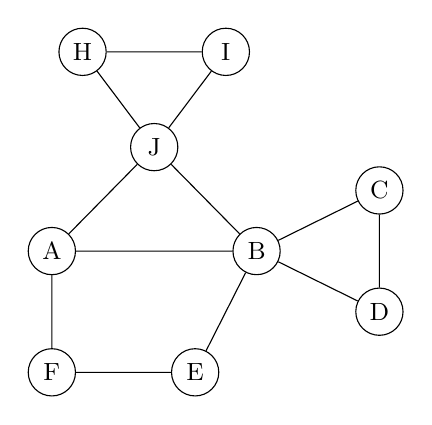
\begin{tikzpicture}[x=1.3cm,y=1.1cm,v/.style={circle,draw,minimum size=6mm,inner sep=1pt,font=\small}]
\node[v] (A) at (0,0) {A};
\node[v] (B) at (2,0) {B};
\node[v] (C) at (3.2,0.7) {C};
\node[v] (D) at (3.2,-0.7) {D};
\node[v] (E) at (1.4,-1.4) {E};
\node[v] (F) at (0,-1.4) {F};
\node[v] (J) at (1,1.2) {J};
\node[v] (H) at (0.3,2.3) {H};
\node[v] (I) at (1.7,2.3) {I};
\draw (A)--(B) (A)--(F) (A)--(J) (B)--(C) (B)--(D) (B)--(E) (B)--(J) (C)--(D) (E)--(F) (J)--(I) (J)--(H) (I)--(H);
\end{tikzpicture}
\end{center}

\textbf{找割點}（資結書第~23.5~節）。 逐一拿掉頂點看圖有沒有斷開：
\begin{itemize}
\item 拿掉 B：C、D 只和 B 相連（還有彼此），和其他頂點分開，B 是割點。
\item 拿掉 J：H、I 只和 J 相連，分開，J 是割點。
\item 拿掉 A：F 經 E 接到 B，J 經 B--J 接到 B，仍然連通，A 不是割點。 其他頂點拿掉也不會斷開。
\end{itemize}
用資結書虛擬碼~23.3 從 A 做 DFS（鄰居依字母順序）也得到同樣的割點 B、J。

\textbf{雙連通元件}（資結書第~23.6~節）是極大的「沒有割點」的子圖，兩個元件最多共用一個割點。
以割點切開：
\begin{itemize}
\item $\{B, C, D\}$：三角形 B--C--D。
\item $\{H, I, J\}$：三角形 J--I--H。
\item $\{A, B, E, F, J\}$：環 A--B--E--F--A 和三角形 A--B--J 共用邊 A--B，兩個環合在同一個元件裡。
\end{itemize}
共三個。 核對：$12$ 條邊各屬一個元件，B--C、B--D、C--D 在第一個，J--I、J--H、I--H 在第二個，
其餘 A--B、A--F、A--J、B--E、B--J、E--F 六條在第三個。

\begin{itemize}
\item (a) 錯：A、B、C、D 不是一個元件，拿掉 B 後 C、D 和 A 分開。
\item (b) 對。
\item (c) 錯：A--B--E--F 這個環還和 J 在同一個元件裡（A--B--J--A 共用邊 A--B），$\{A, B, E, F\}$ 不是
極大的。
\item (d) 照字面錯：圖裡沒有 G。 （若是 $\{J, H, I\}$ 則對，見第一段。）
\item (e) 錯，(b) 對。
\end{itemize}
\end{pastsoln}
